\chapter{Documentation}
Documentation is something commonly taken too lightly. The legacy panel system
contains little to no documentation.
This frustrates developers and inhibits any changes to the codebase, because
there might be this undocumented flow of code that will break and only found out
about much later.

Fortunately there are some tools not only to properly write documentation
, but also to encourage developers to write documentation as the codebase
evolves.

\section{Inline documentation}
Documentation regarding the description code itself is kept close to the code,
in the form of inline documentation.

This means most of the documentation will be housed along with with the source
code itself. The goal is to minimize separation of code and documentation as
this easily leads to inconsistencies between the two.

Advantages of inline documentation are the reduced chances for outdated
documentation and being able to enrich source code with typed annotations
\cite{JS_Annotations}.

Source code consists of C++, JavaScript, HTML, and CSS code. The inline
documentation described here is applicable to the last three.

\subsection{JSDocs}
The syntax used to document JavaScript code is called JSDocs and is currently
at version 3\cite{JS_Annotations}\cite{JSDoc}. It provides us with a rich set of expressions
enabling a developer to write documentation comparable to JavaDoc.

JSDocs has wide industry adoption for JavaScript projects. It is widely used to
make code more understandable, generate HTML documentation, or use it to generate
the large traditional developer manuals.

In addition to JSDocs there are specific points in the source code where a developer can
provide code examples and extra directives to document HTML and CSS code. This
is however a non-standard method since there is no standardized way to document
any of the other languages inline.

\section{Global level}
The global level is the highest level and is the only level where documentation
is separated from the source code.

\subsection{Goals}
The main purpose of this documentation level is to be an entry point for developers.
It will teach developers the basics of the codebase, why things need to be done
one way or the other, and will point them to lower-level documentation whenever
appropriate (such as which package or element could be useful for a particular
use case).

Where lower level documentation will only focus on how to get stuff done, this
documentation level also has the responsibility to show developers concepts like
Separation of Concerns (see chapter \ref{Separation of Concerns}) and modular thinking.

\subsection{Sphinx}
This global documentation level is built using Sphinx (\url{http://www.sphinx-doc.org/}).
It takes a set of wiki-like documents and converts them in various types of
resources (HTML, \LaTeX, \ldots).
This is primarily focused on HTML output, but the \LaTeX~version is included in
this document as appendix~\ref{appendix_sphinx}.

\label{Sphinx}

\section{Package level}
The global level gives an overview of the packages that are available to a panel
developer.
The package level lies under the global level and is the first automatically
generated level. It describes the package's content and its capabilities.

\subsection{Goals}
Primarily, this documentation level gives a quick overview of the content of a
package. It also points readers to additional resources like element-level
documentation, the repository where the source code is hosted, and live demos
where supported.

\subsection{Grunt}
This documentation is generated in the Grunt build cycle described in chapter
\ref{Grunt build system}.
It loads and interprets every component of the package and generates a summary
page giving a general overview and pointing to several useful resources for each
component such as the documentation on the element level, a link to the code
repository, and a link to a live demo of the component if available.

The code it uses to render this documentation is housed in the source code of
each component. It gets interpreted by Grunt and is then compiled in the package
documentation page.

An example of a package level documentation page is show in figure \ref{fig:packagedocumentation}.
\begin{figure}
  \centering
  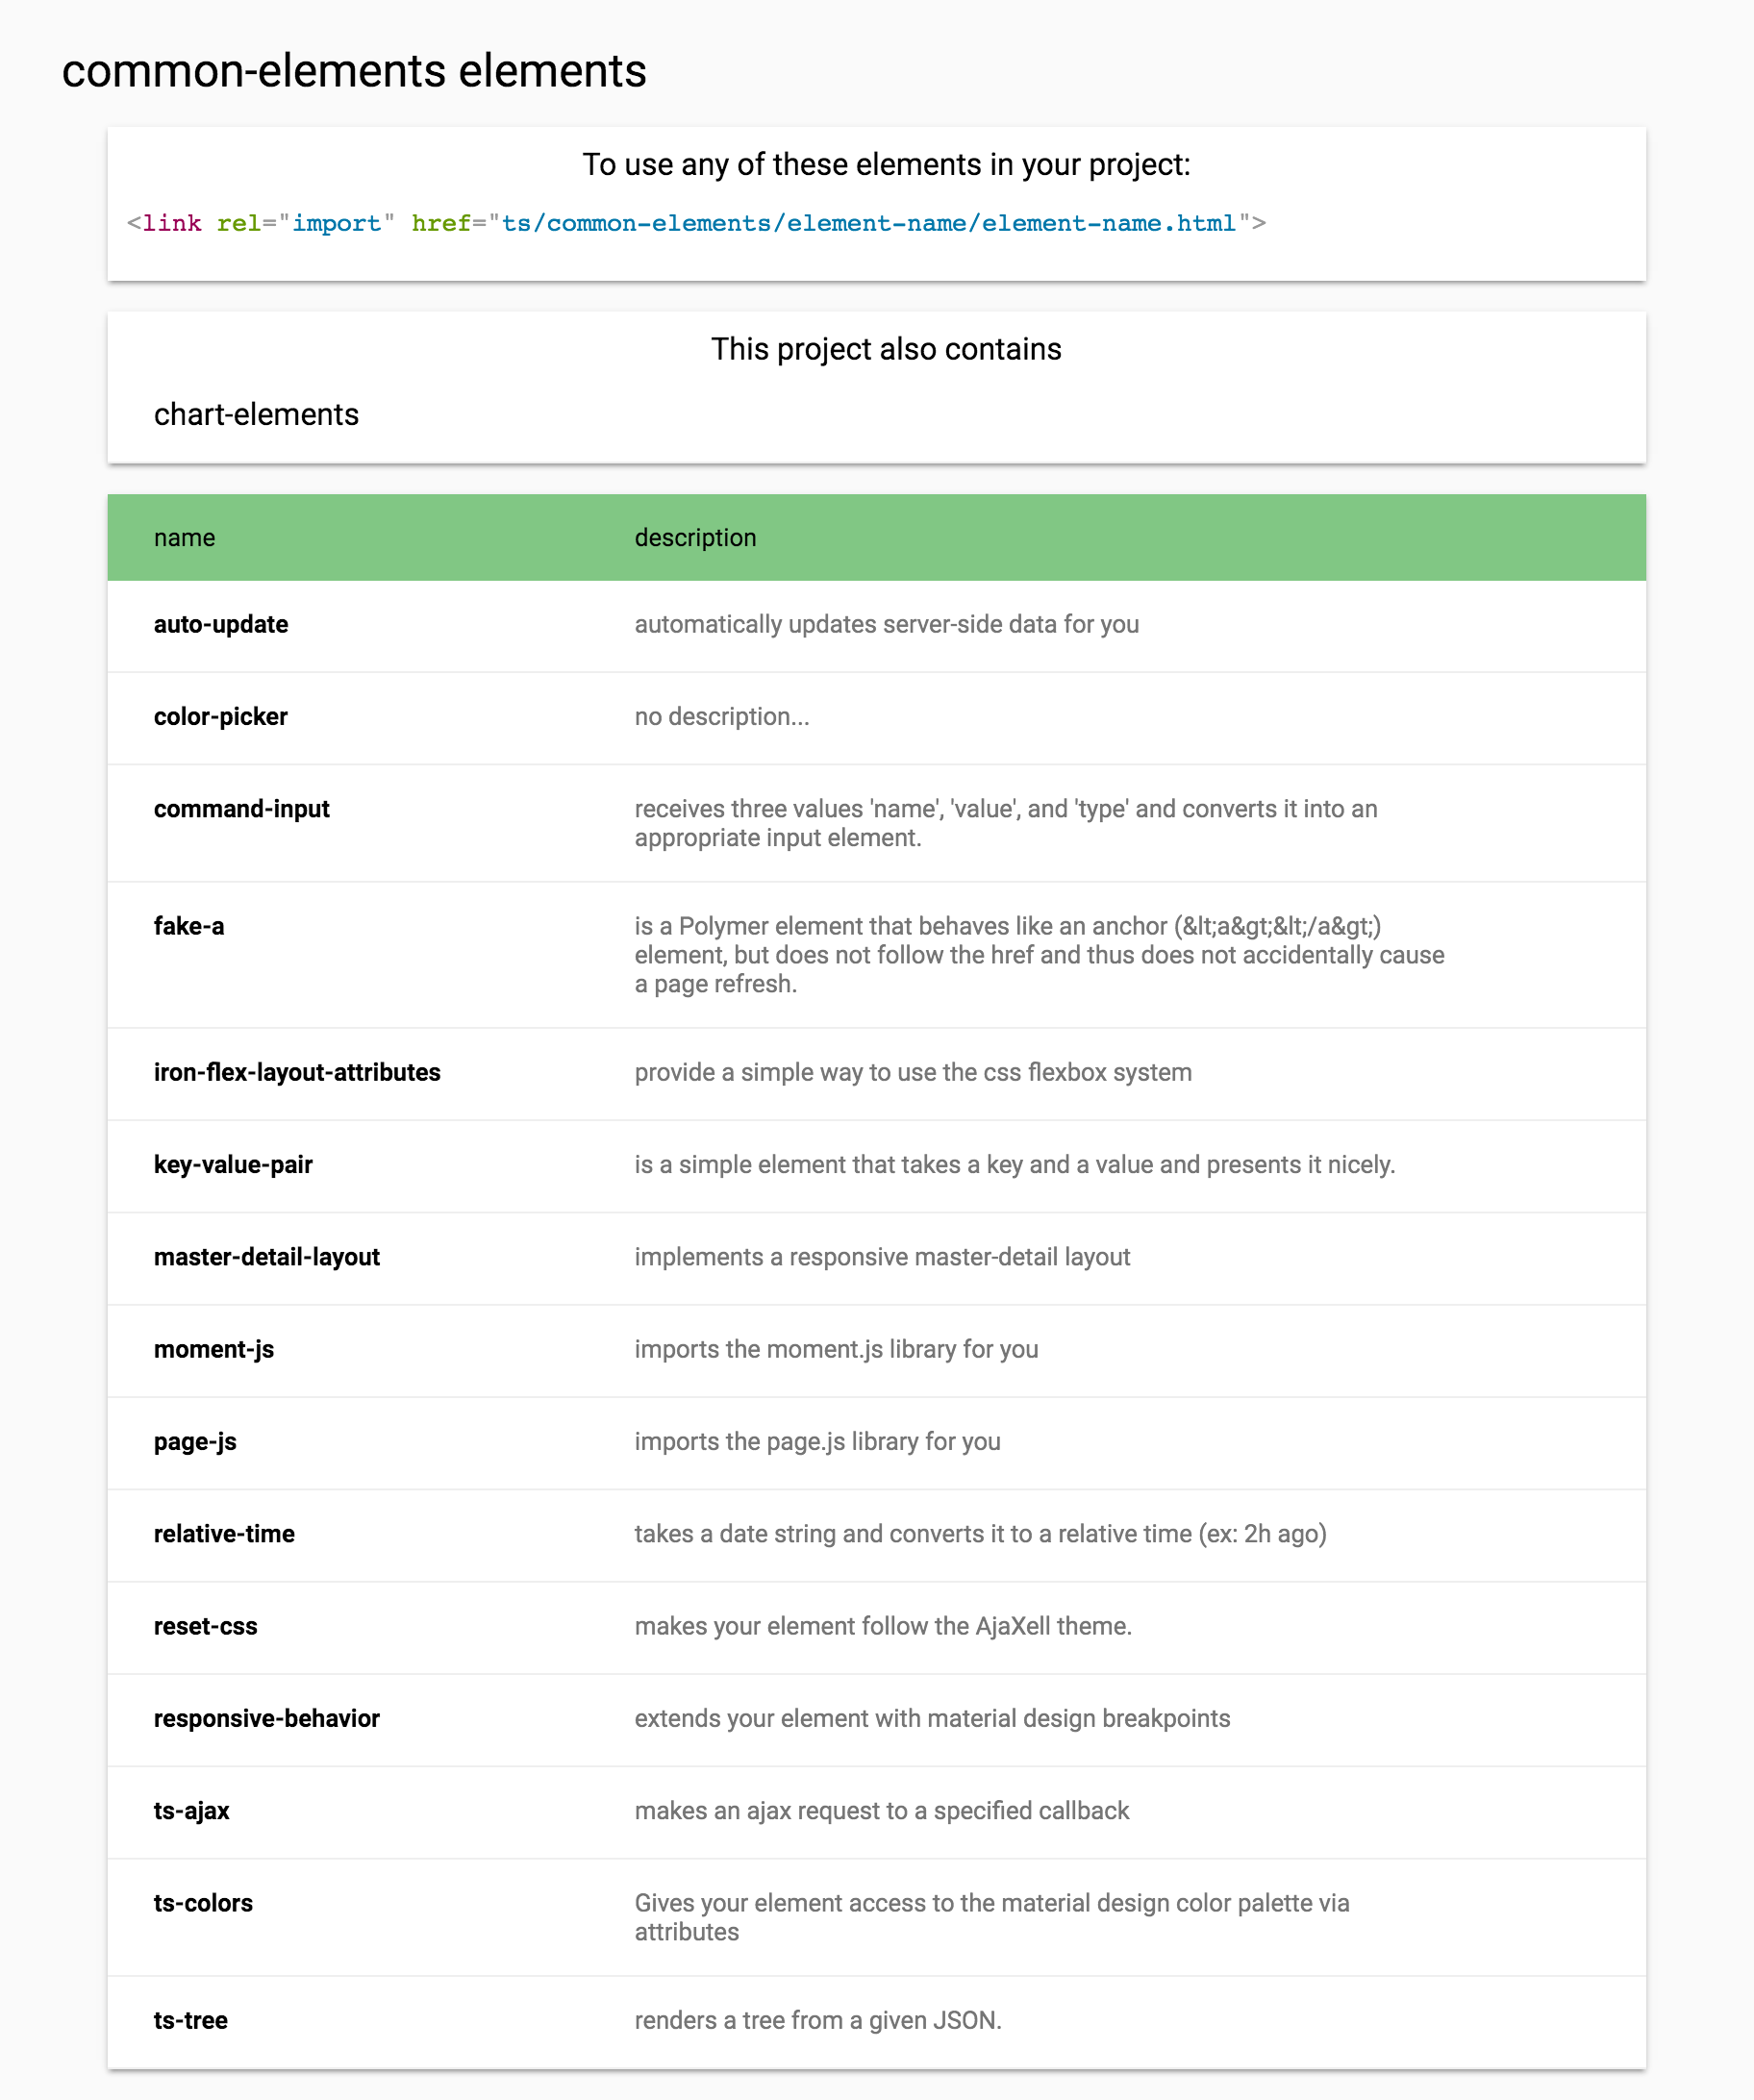
\includegraphics[width=\textwidth]{images/package-documentation}
  \caption{Documentation page of the common-elements package}
  \label{fig:packagedocumentation}
\end{figure}

\section{Element level}
The lowest level of documentation is documentation of individual web components.
This level is also auto-documented from the component's source code.
But unlike the documentation on the package level, where documentation is
generated on compile time, the documentation here is rendered on the fly, client-side.


\subsection{Goals}
This documentation provides an overview of all the properties and available
calls of this component. It can also provide code examples and even live
demos.

\subsection{iron-component-page}
Client-side rendering is done by using a specialized web component called `iron-component-page`
(\url{https://elements.polymer-project.org/elements/iron-component-page}).
It uses the `hydrolysis.js` library to interpret the inline documentation provided
by the developer in the source code of the web component, and compiles this into
a documentation page.

An example of an element level documentation page is show in figure \ref{fig:elementdocumentation}.
\begin{figure}
  \centering
  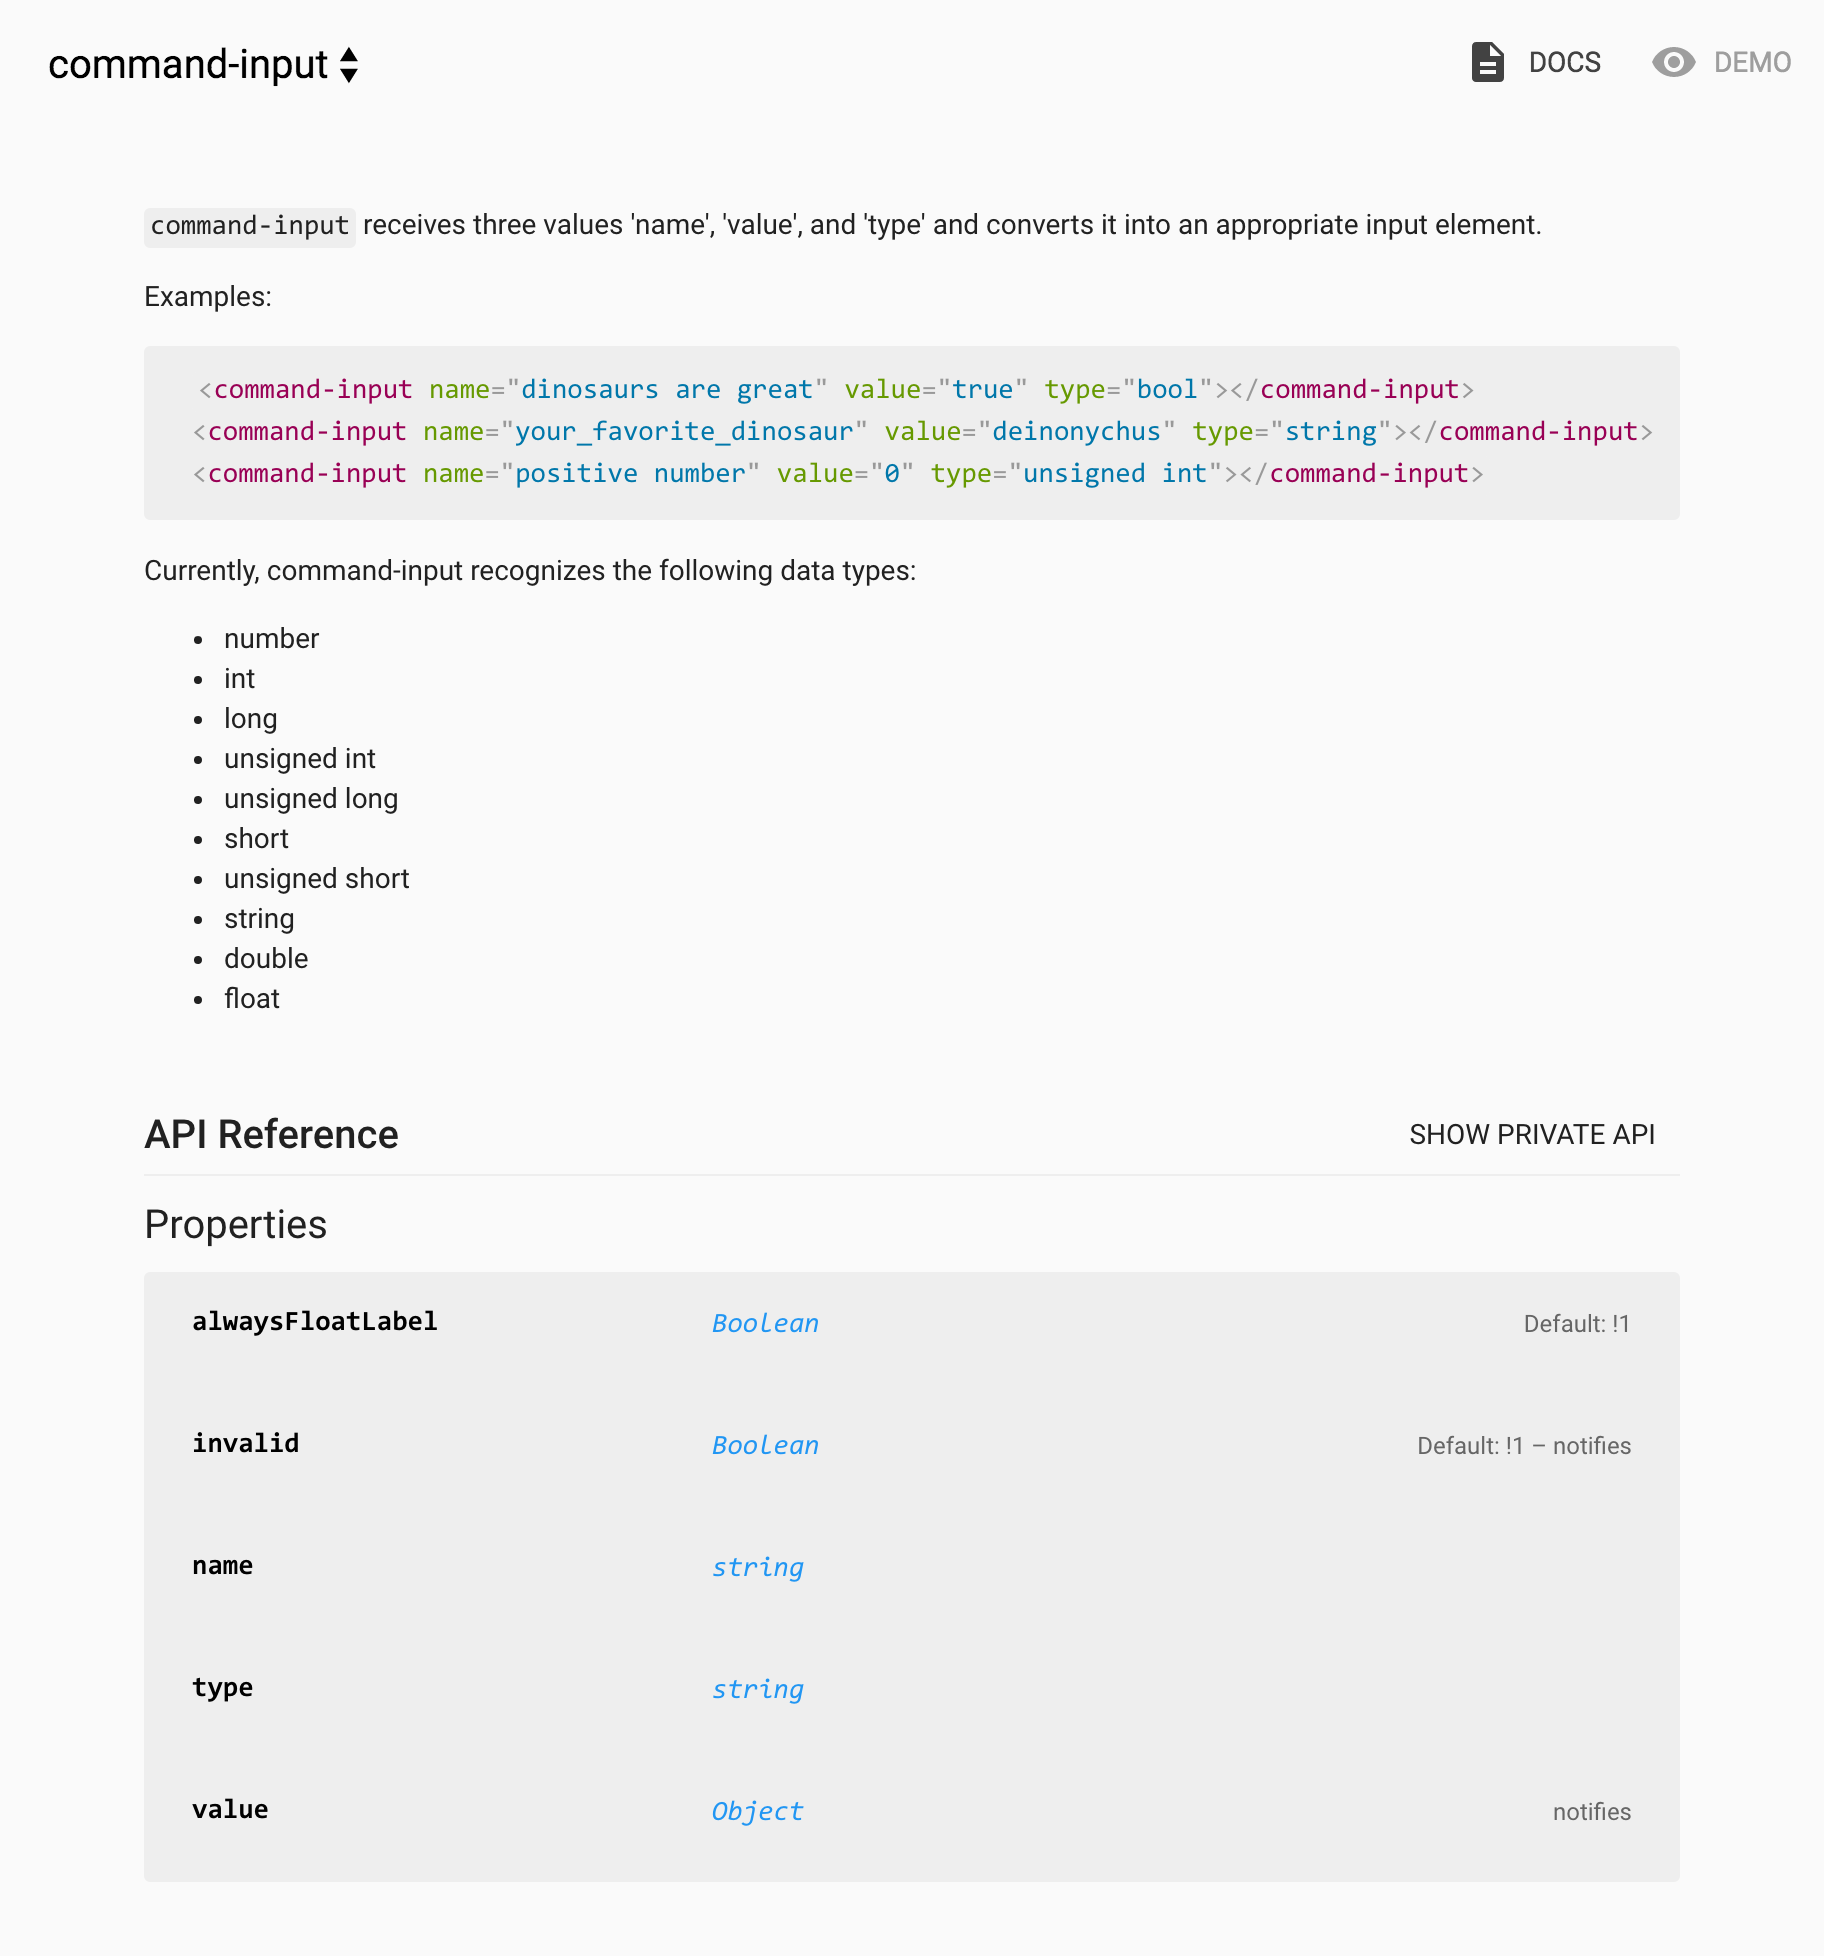
\includegraphics[width=\textwidth]{images/element-documentation}
  \caption{Documentation page of the command-input element}
  \label{fig:elementdocumentation}
\end{figure}
